% 由 tutorial.tex 自动拆分为第 16 章
\chapter{结果可视化与落地}
\section{加载生产权重：一致性散点}

把本项目训练好的权重（BC+DAgger，闭环 $100\%$）装进 numpy 版，在 $512$ 个真实窗口上比较：

\begin{center}
\small
\begin{tabular}{@{}lcc@{}}
\toprule
指标 & 数值 & 说明 \\
\midrule
$\max|u_{\text{numpy}}-u_{\text{torch}}|$ & $5.4\times10^{-6}$\,N & float32 权重下 \\
平均偏差 & $8.1\times10^{-7}$\,N & $u_{\max}$ 的 $0.0000067\%$ \\
相关系数 & $1.000000000$ & -- \\
\midrule
闭环成功率（numpy 策略，30 组初值） & $30/30$ & 与 torch 版完全一致 \\
从下垂出发摆起用时 & $1.9$\,s & -- \\
\bottomrule
\end{tabular}
\end{center}

\begin{figure}[htbp]
\centering
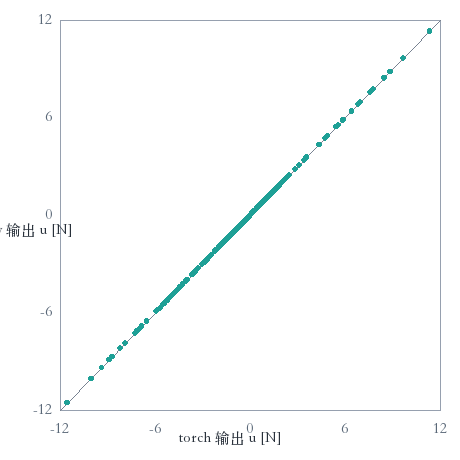
\includegraphics[width=0.42\linewidth]{fig_parity.png}
\caption{numpy 与 torch 在同一批真实窗口上的输出。所有点落在 $y=x$ 上。}
\end{figure}

\section{注意力热图}

\begin{figure}[htbp]
\centering
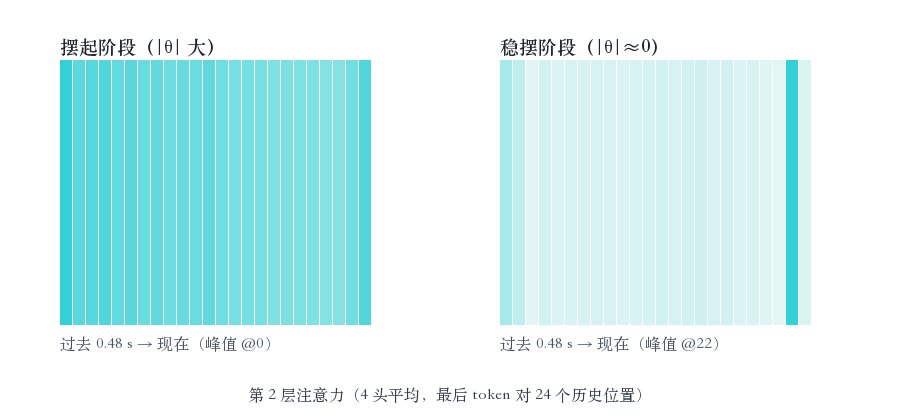
\includegraphics[width=0.96\linewidth]{fig_attention.png}
\caption{第 2 层注意力（4 头平均，最后 token 对 24 个历史位置）。
左：摆起阶段，权重铺满整段（峰值偏早）；右：稳摆阶段，峰值锁在最近第 2 步。
这是"估相位"与"估变化率"两种信息需求的直接体现。}
\end{figure}

\section{梯度量级}

\begin{figure}[htbp]
\centering
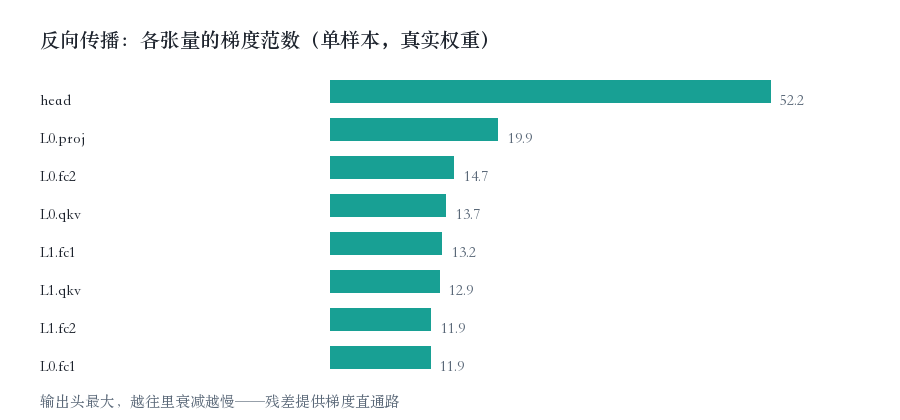
\includegraphics[width=0.8\linewidth]{fig_grad.png}
\caption{反向传播中各张量的梯度范数（真实权重、单样本）。输出头最大，越往里衰减越慢
——残差提供了梯度直通路。}
\end{figure}


本教程的模型与项目里部署的控制器是同一个结构。把它变成控制器的全部差别只有三处：

\begin{enumerate}[leftmargin=1.6em,itemsep=3pt]
  \item \textbf{输入特征}：$F=6$，即 $[\sin\theta,\cos\theta,\dot\theta/4,\dot p/4,p/2.4,u_{k-1}/12]$，
        全部归一化到 $[-2,2]$；
  \item \textbf{窗口}：$T=24$（$0.48$\,s @ 50\,Hz），覆盖约 $1/3$ 个摆动周期；
  \item \textbf{输出限幅}：$u=12\tanh(\cdot)$，天然落在执行器的 $\pm12$\,N 内。
\end{enumerate}

部署时把它量化到 int8（$71$\,KB $\to$ $16.6$\,KB），单点最大误差 $0.14$\,N；
浏览器里手写前向（LayerNorm $\to$ 多头因果注意力 $\to$ GELU $\to\tanh$）单步 $0.32$\,ms。
手写前向之所以敢用，正是因为本教程这套"逐层对齐"的验证方法。

